\section{Results}
\subsection{$H_{1a}$ and $H_{1b}$}

To test $H_{1a}$, I first establish a model with 50 agents, 5 issues, and an
openness parameter of 0.40. In order to measure the impact of varying edge
probability on average assortativity across all issues, I ran each combination
of parameters 20 times starting with an edge probability of 0.05 and ending
with an edge probability of 0.95, in increments of .05. The results of this
model run are shown in Figure~\ref{H1a_plot}.

\begin{figure}
\centering
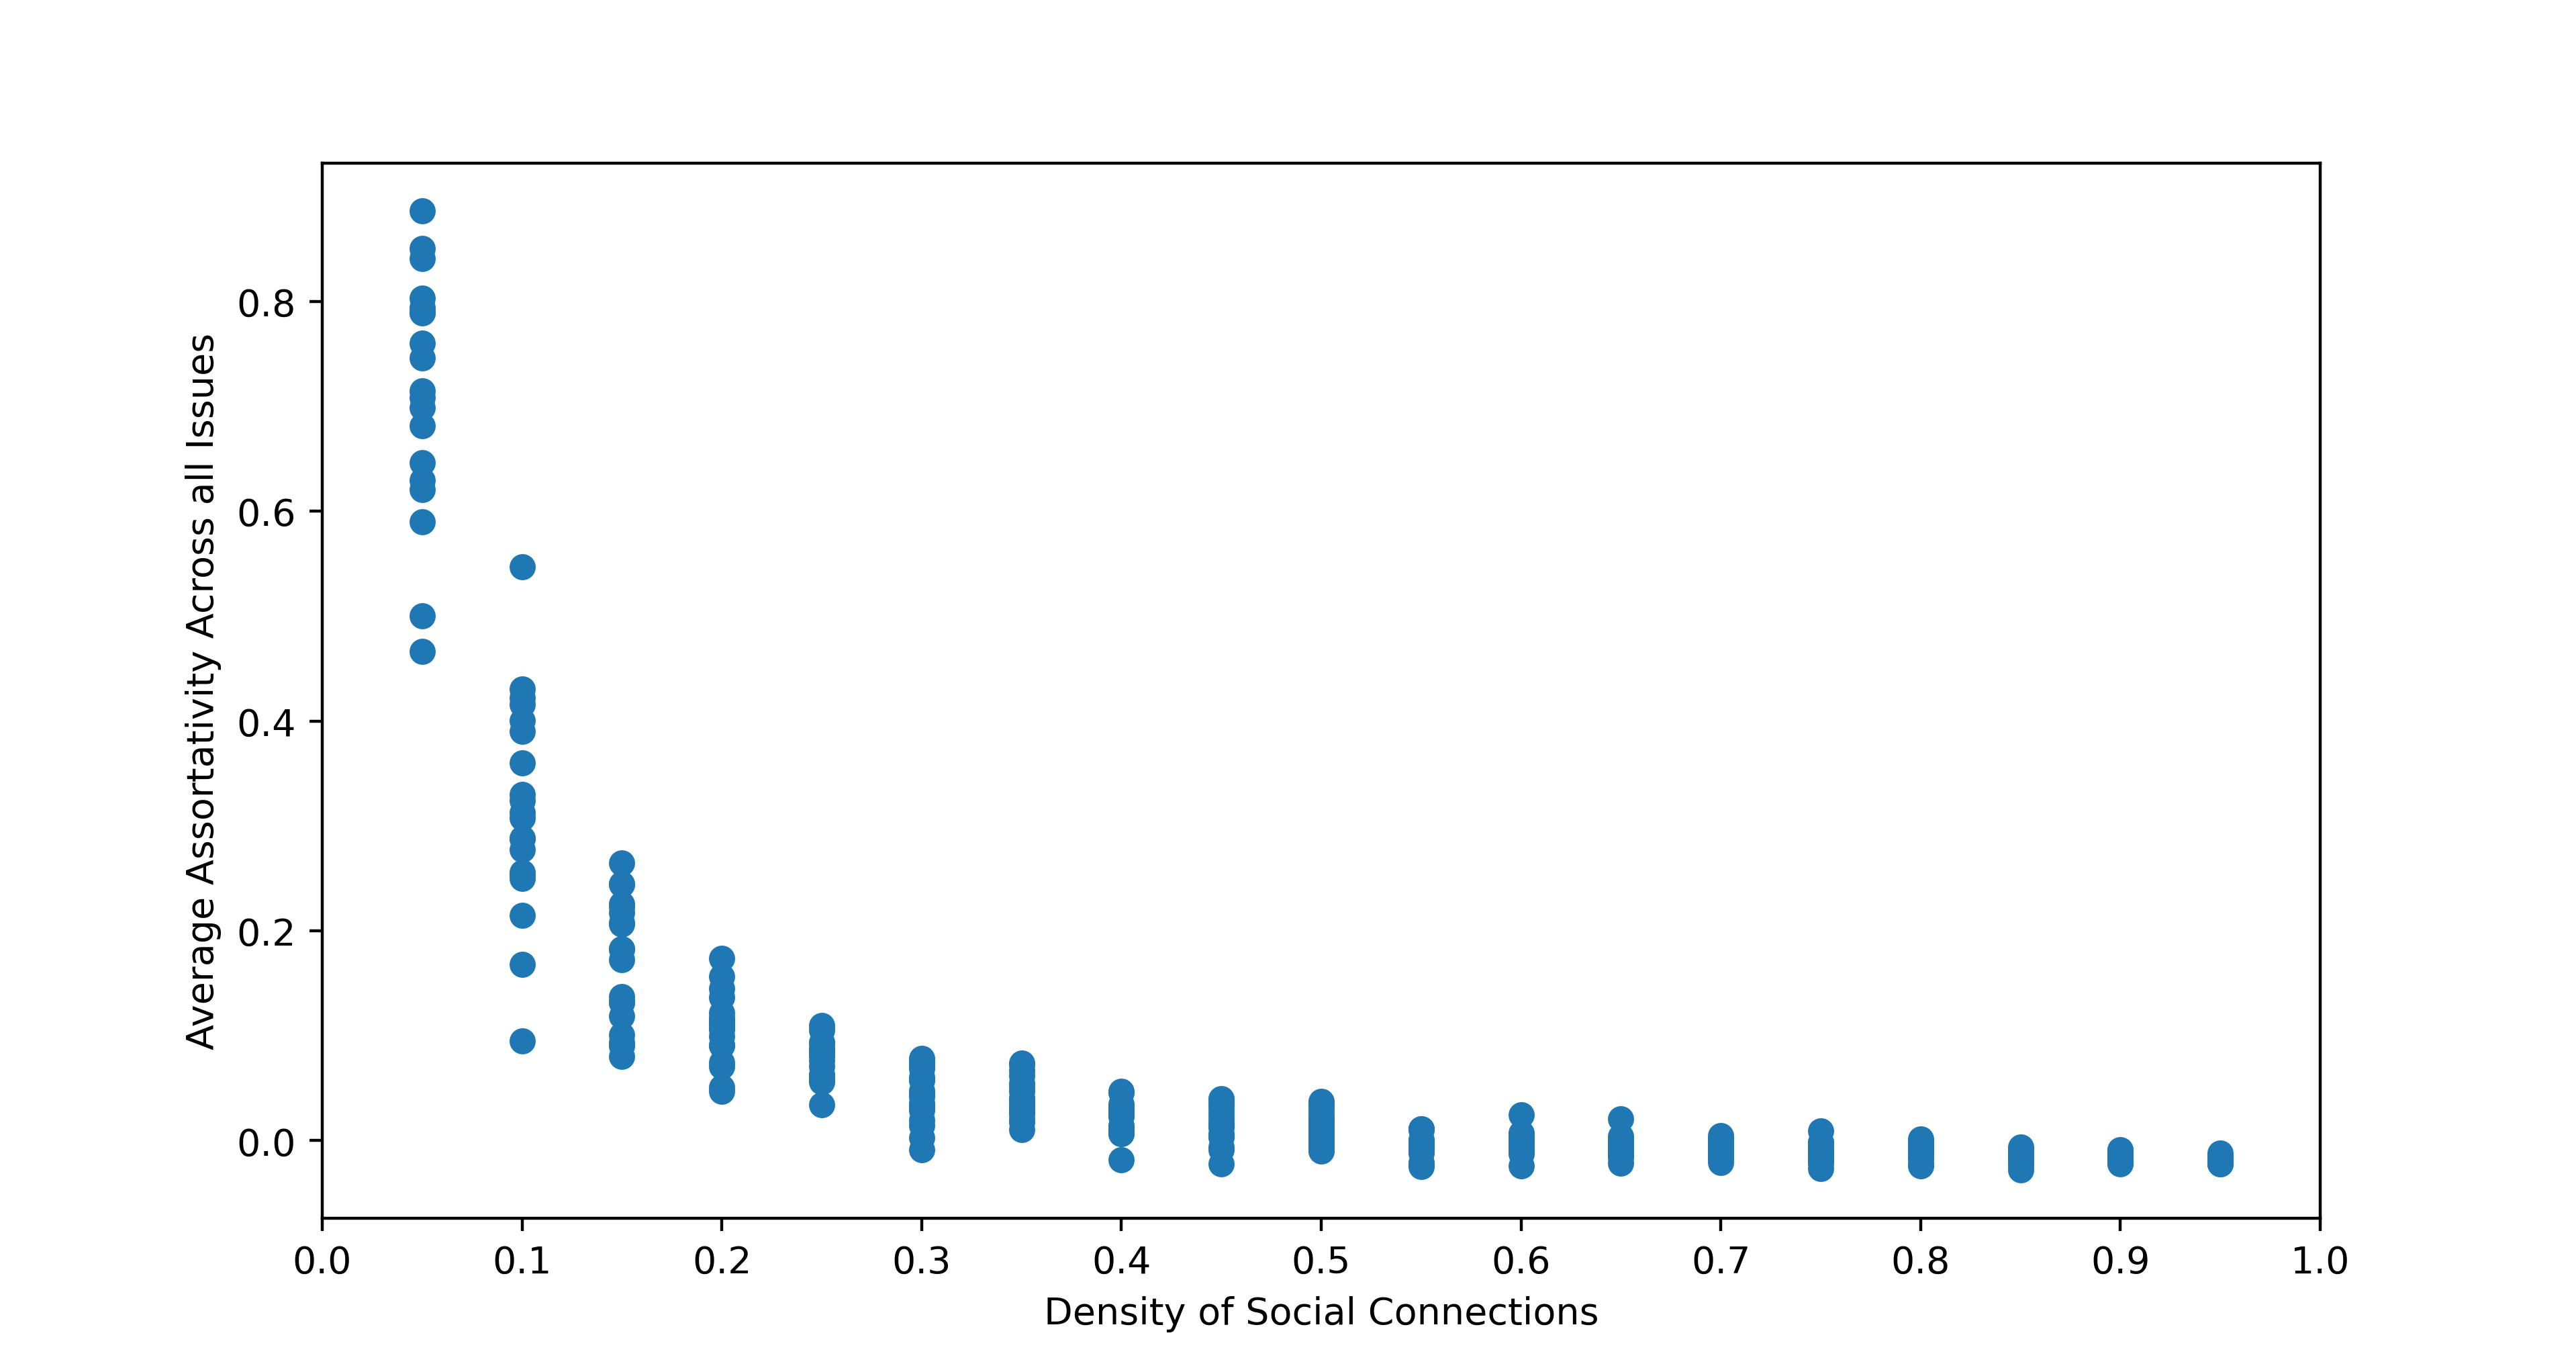
\includegraphics[width=1.0\columnwidth]{./Graphs/Assort_edge.png}
\caption{Average Assortativity across all Issues and Edge Probability}
\label{H1a_plot}
\end{figure}

From the graph, we see that as the edge probability (or density of social connections)
increases, the average assortativity across all issues decreases. This is the
exact opposite of my hypothesis. One possible explanation for this result is
that when connections are more dense, there is a higher chance that agents will
be exposed to a more diverse set of opinions. There is thus a higher chance
that agents will be pulled to the `average` opinion for a given issue, which
would produce lower assortativity. With less densely connected social networks, it is easier for an individual to get stuck in an echo chamber that has a low overall diversity of opinions. In the aggregate, this would produce a social network with higher assortativity. From this result, I am able to infer
that societies where individuals are more densely connected may experience
less polarization than more sparsely-connected societies do. 

In addition to the negative correlation between density of social connections
and polarization, I also noticed that the relationship between these two variables
appears negative-exponential in nature. The variance was too high, however, for
me to draw a solid conclusion on whether the relationship truly conforms to a
negative-exponential, a power-law, or any other standard distribution.

To test $H_{1b}$, I first establish a model with 50 agents, 5 issues, and an
edge probability of 0.50. In order to measure the impact of varying the
openness threshold on average assortativity across all issues, I ran each
combination of inputs 20 times with an openness parameter ranging from 0.05 to
0.95 in increments of .05. The results of this model run are shown in
Figure~\ref{H1b_plot}. As is depicted, there is no obvious relationship at all
between the openness threshold and the average assortativity across all issues. 

\begin{figure}
\centering
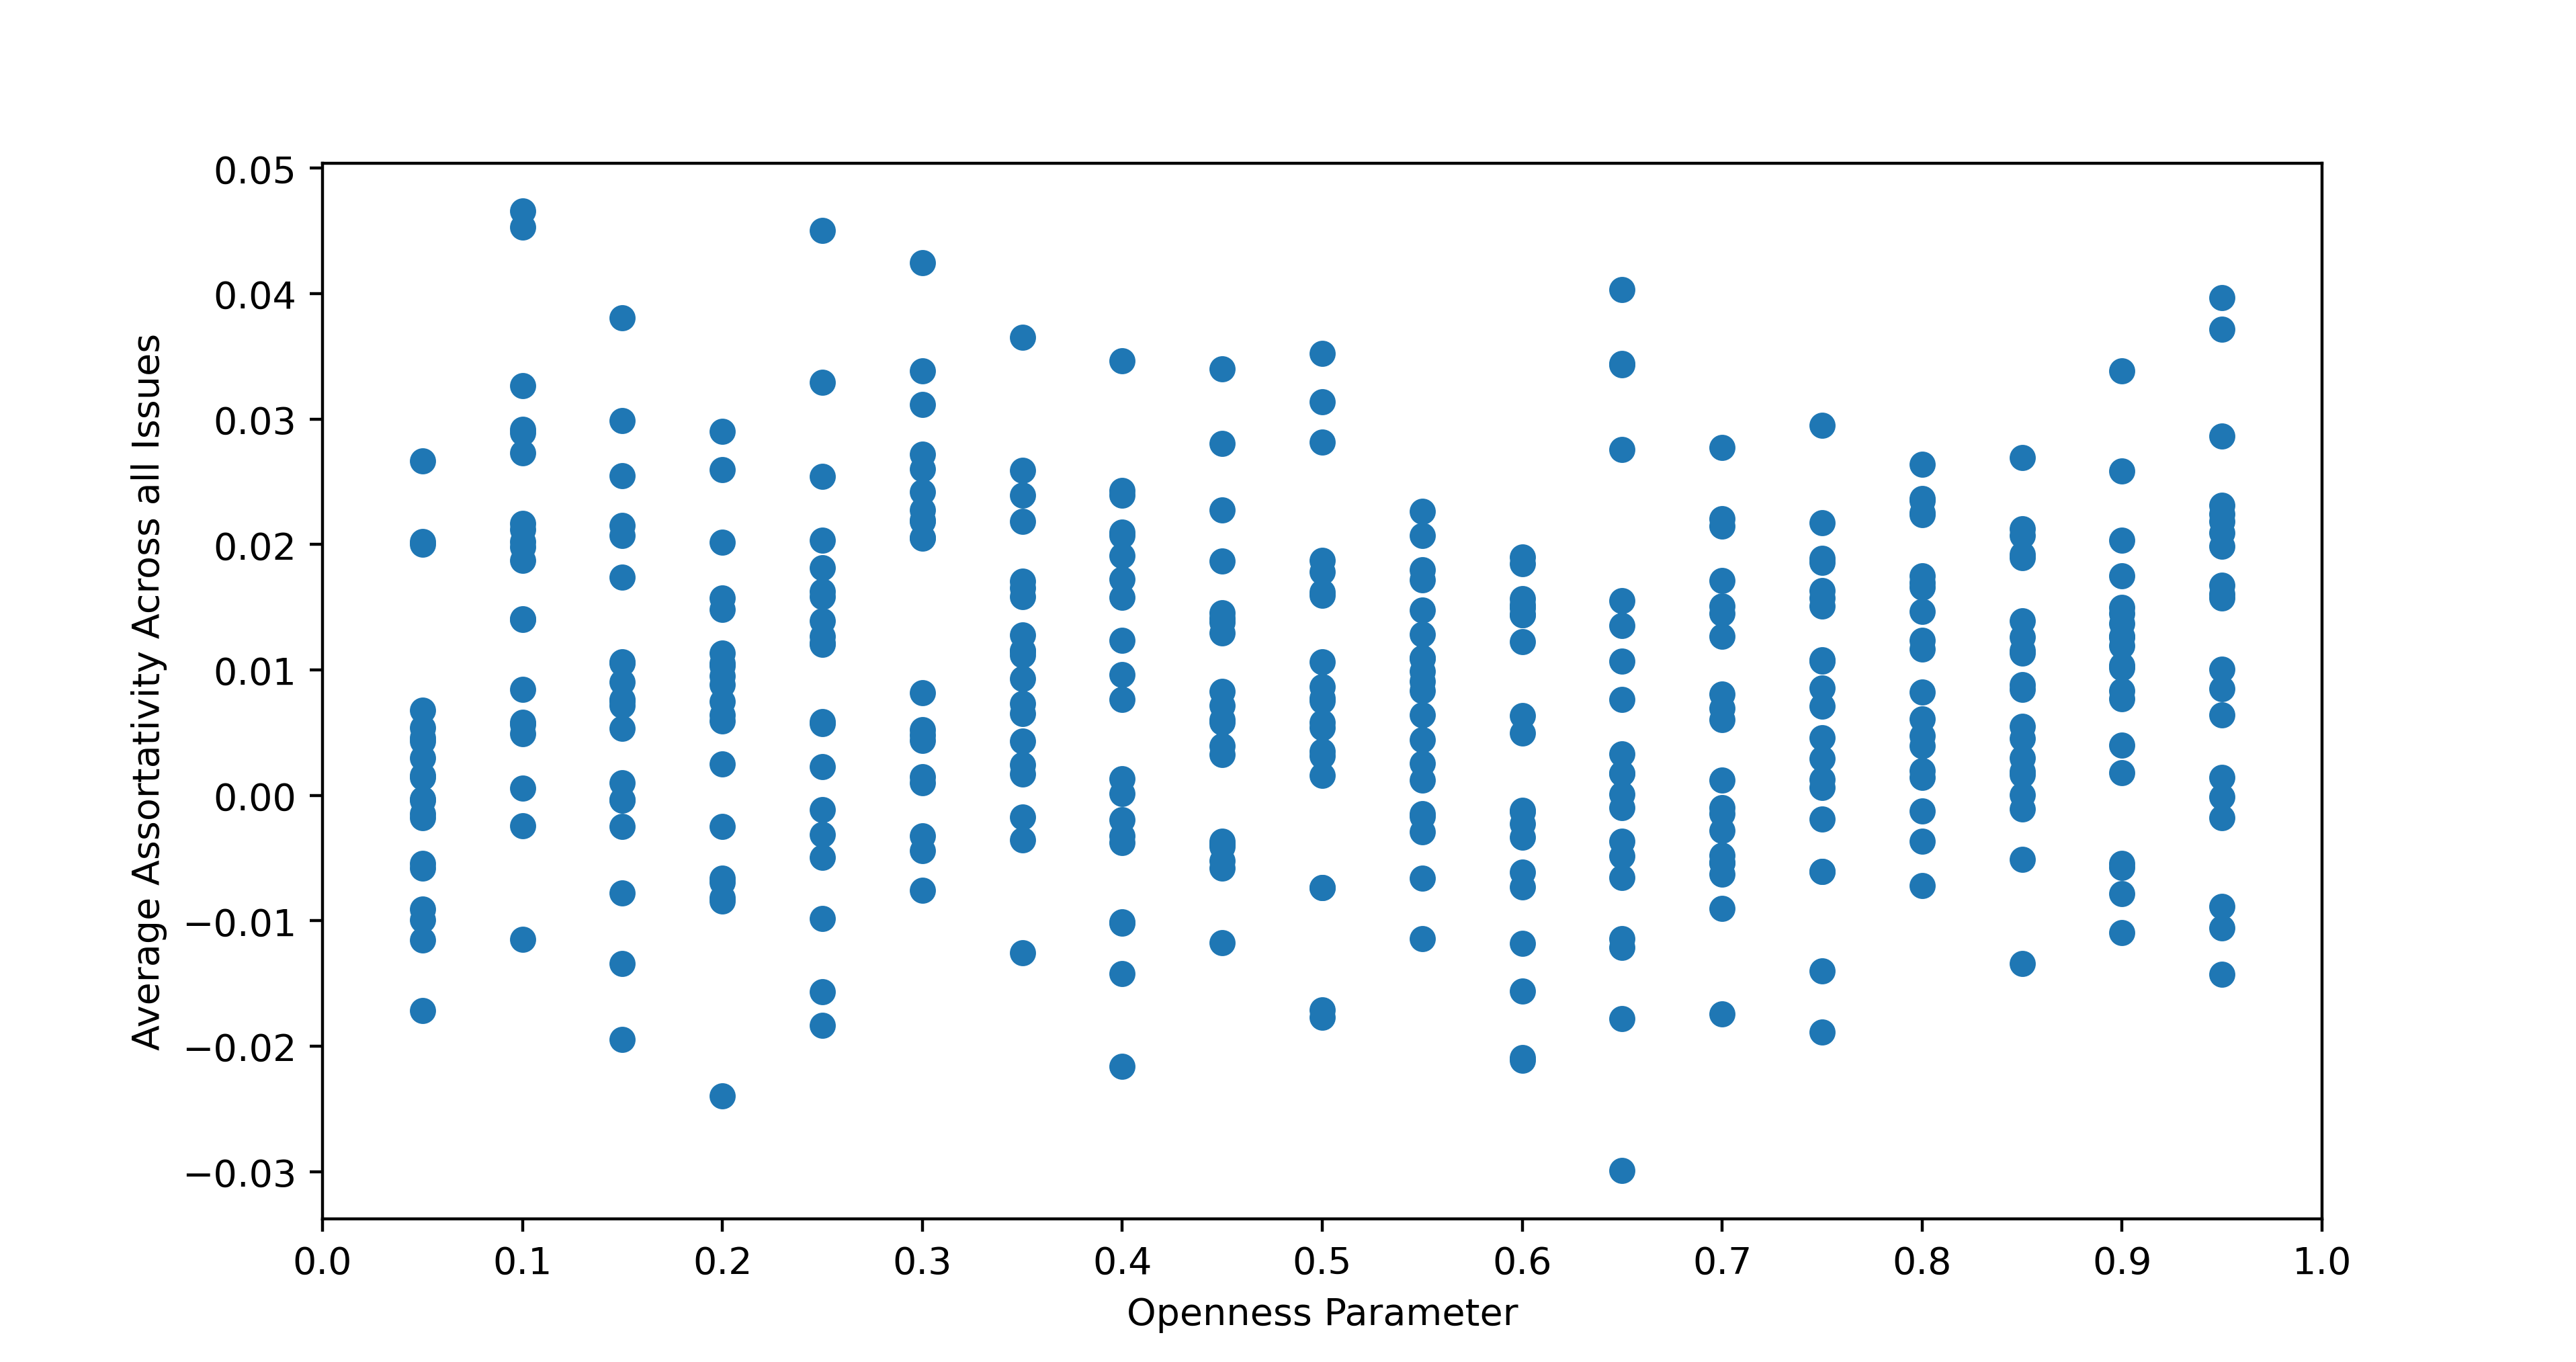
\includegraphics[width=1.0\columnwidth]{./Graphs/Assort_openness.png}
\caption{Average Assortativity across all Issues and Openness Threshold}
\label{H1b_plot}
\end{figure}

This is an interesting result. Agents in the model are influenced when they are
close in opinion (within the openness threshold) to another agent on the same
issue. Therefore, I believed that openness would play a role in determining the assortativity of a society. 
It should be noted that I tested this hypothesis with multiple different values of the edge probability (0.15,
0.40, and 0.50), to ensure that the edge probability was not having an impact
on the results. Even still, I hope to investigate this hypothesis further in future research. 

\subsection{$H_{2a}$ and $H_{2b}$}

To test $H_{2a}$, I establish a model with 50 agents, 5 issues, and an
openness threshold of 0.30. First, I ran a parameter sweep varying the edge
probability from 0.05 to 0.95 to measure the impact of this parameter on the
number of opinion clusters. The results of this parameter sweep are shown in
Figure~\ref{H2a_plot_big}.

\begin{figure}
\centering
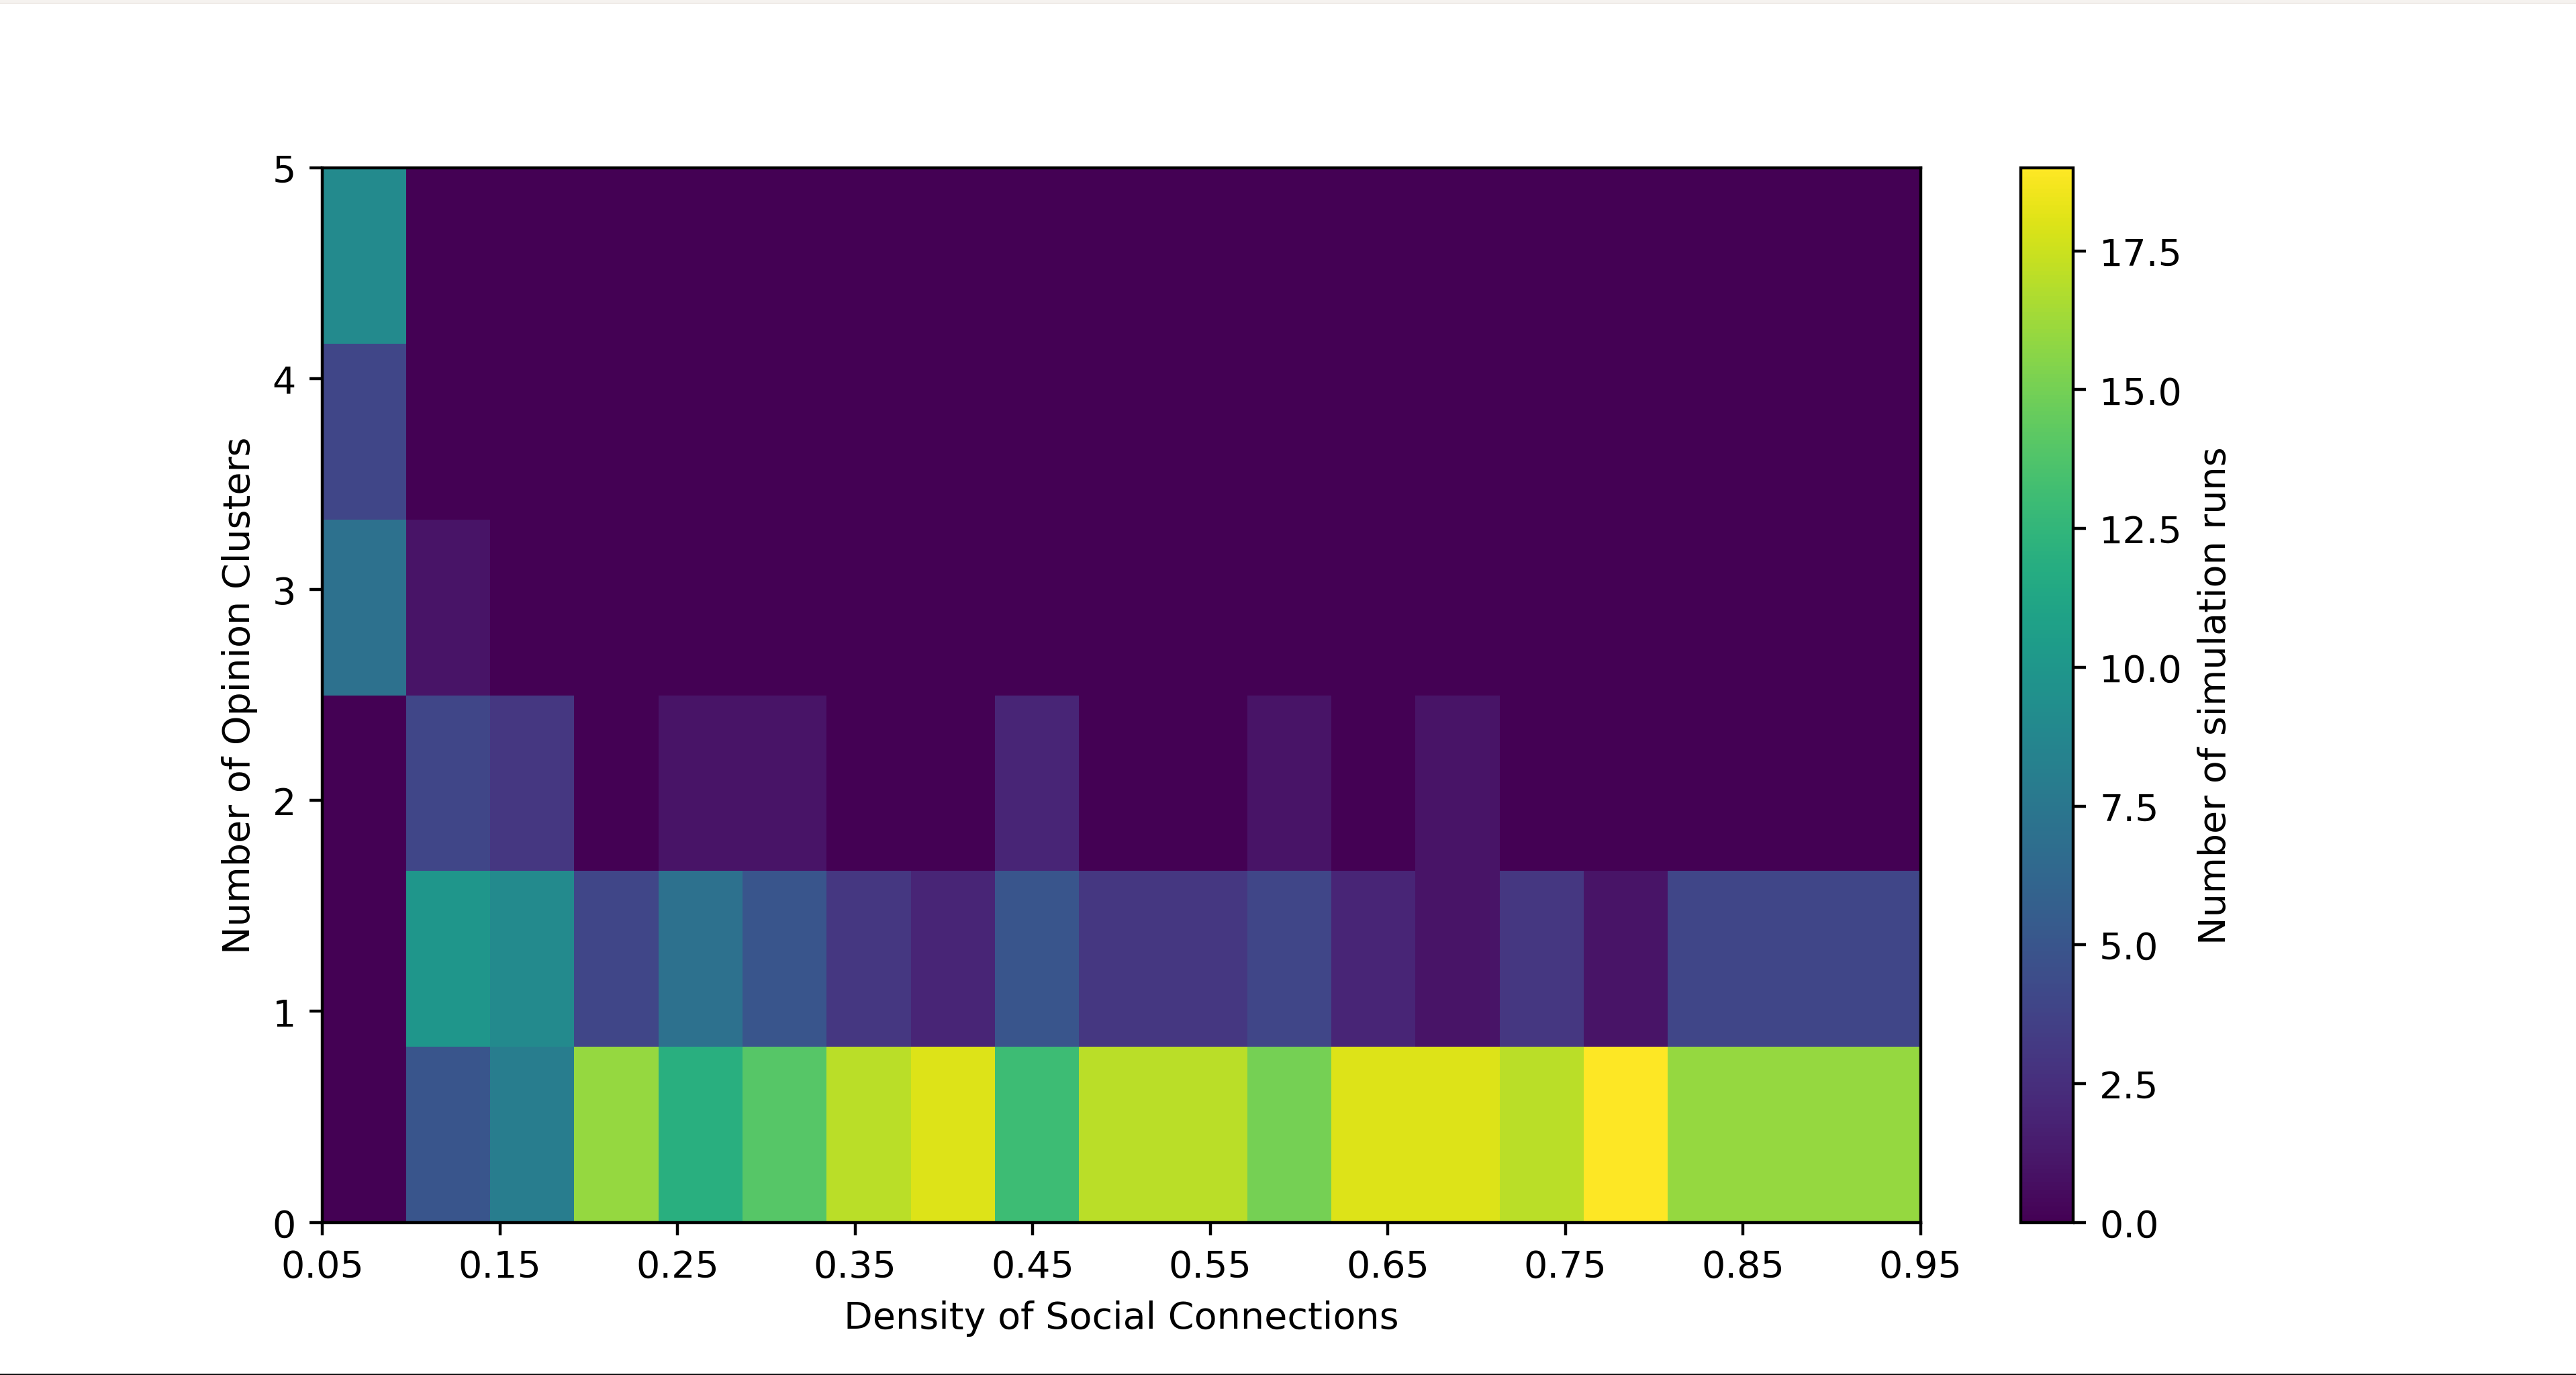
\includegraphics[width=1.0\columnwidth]{./Graphs/ClusterEdge/Cluster_edgeBig.png}
\caption{Number of Opinion Clusters and Edge Probability (0.05 - 0.95)}
\label{H2a_plot_big}
\end{figure}

I noticed that as with $H_{2a}$, there appears to be a tipping point with the
number of opinion clusters and the edge probability. To further explore this
hypothesis, I ran another parameter sweep, this time varying the edge
probability from 0.05 to 0.40 incrementing by 0.01 for each suite of 20 model
runs. The results of this parameter sweep are depicted in
Figure~\ref{H2a_plot_small}.

\begin{figure}
\centering
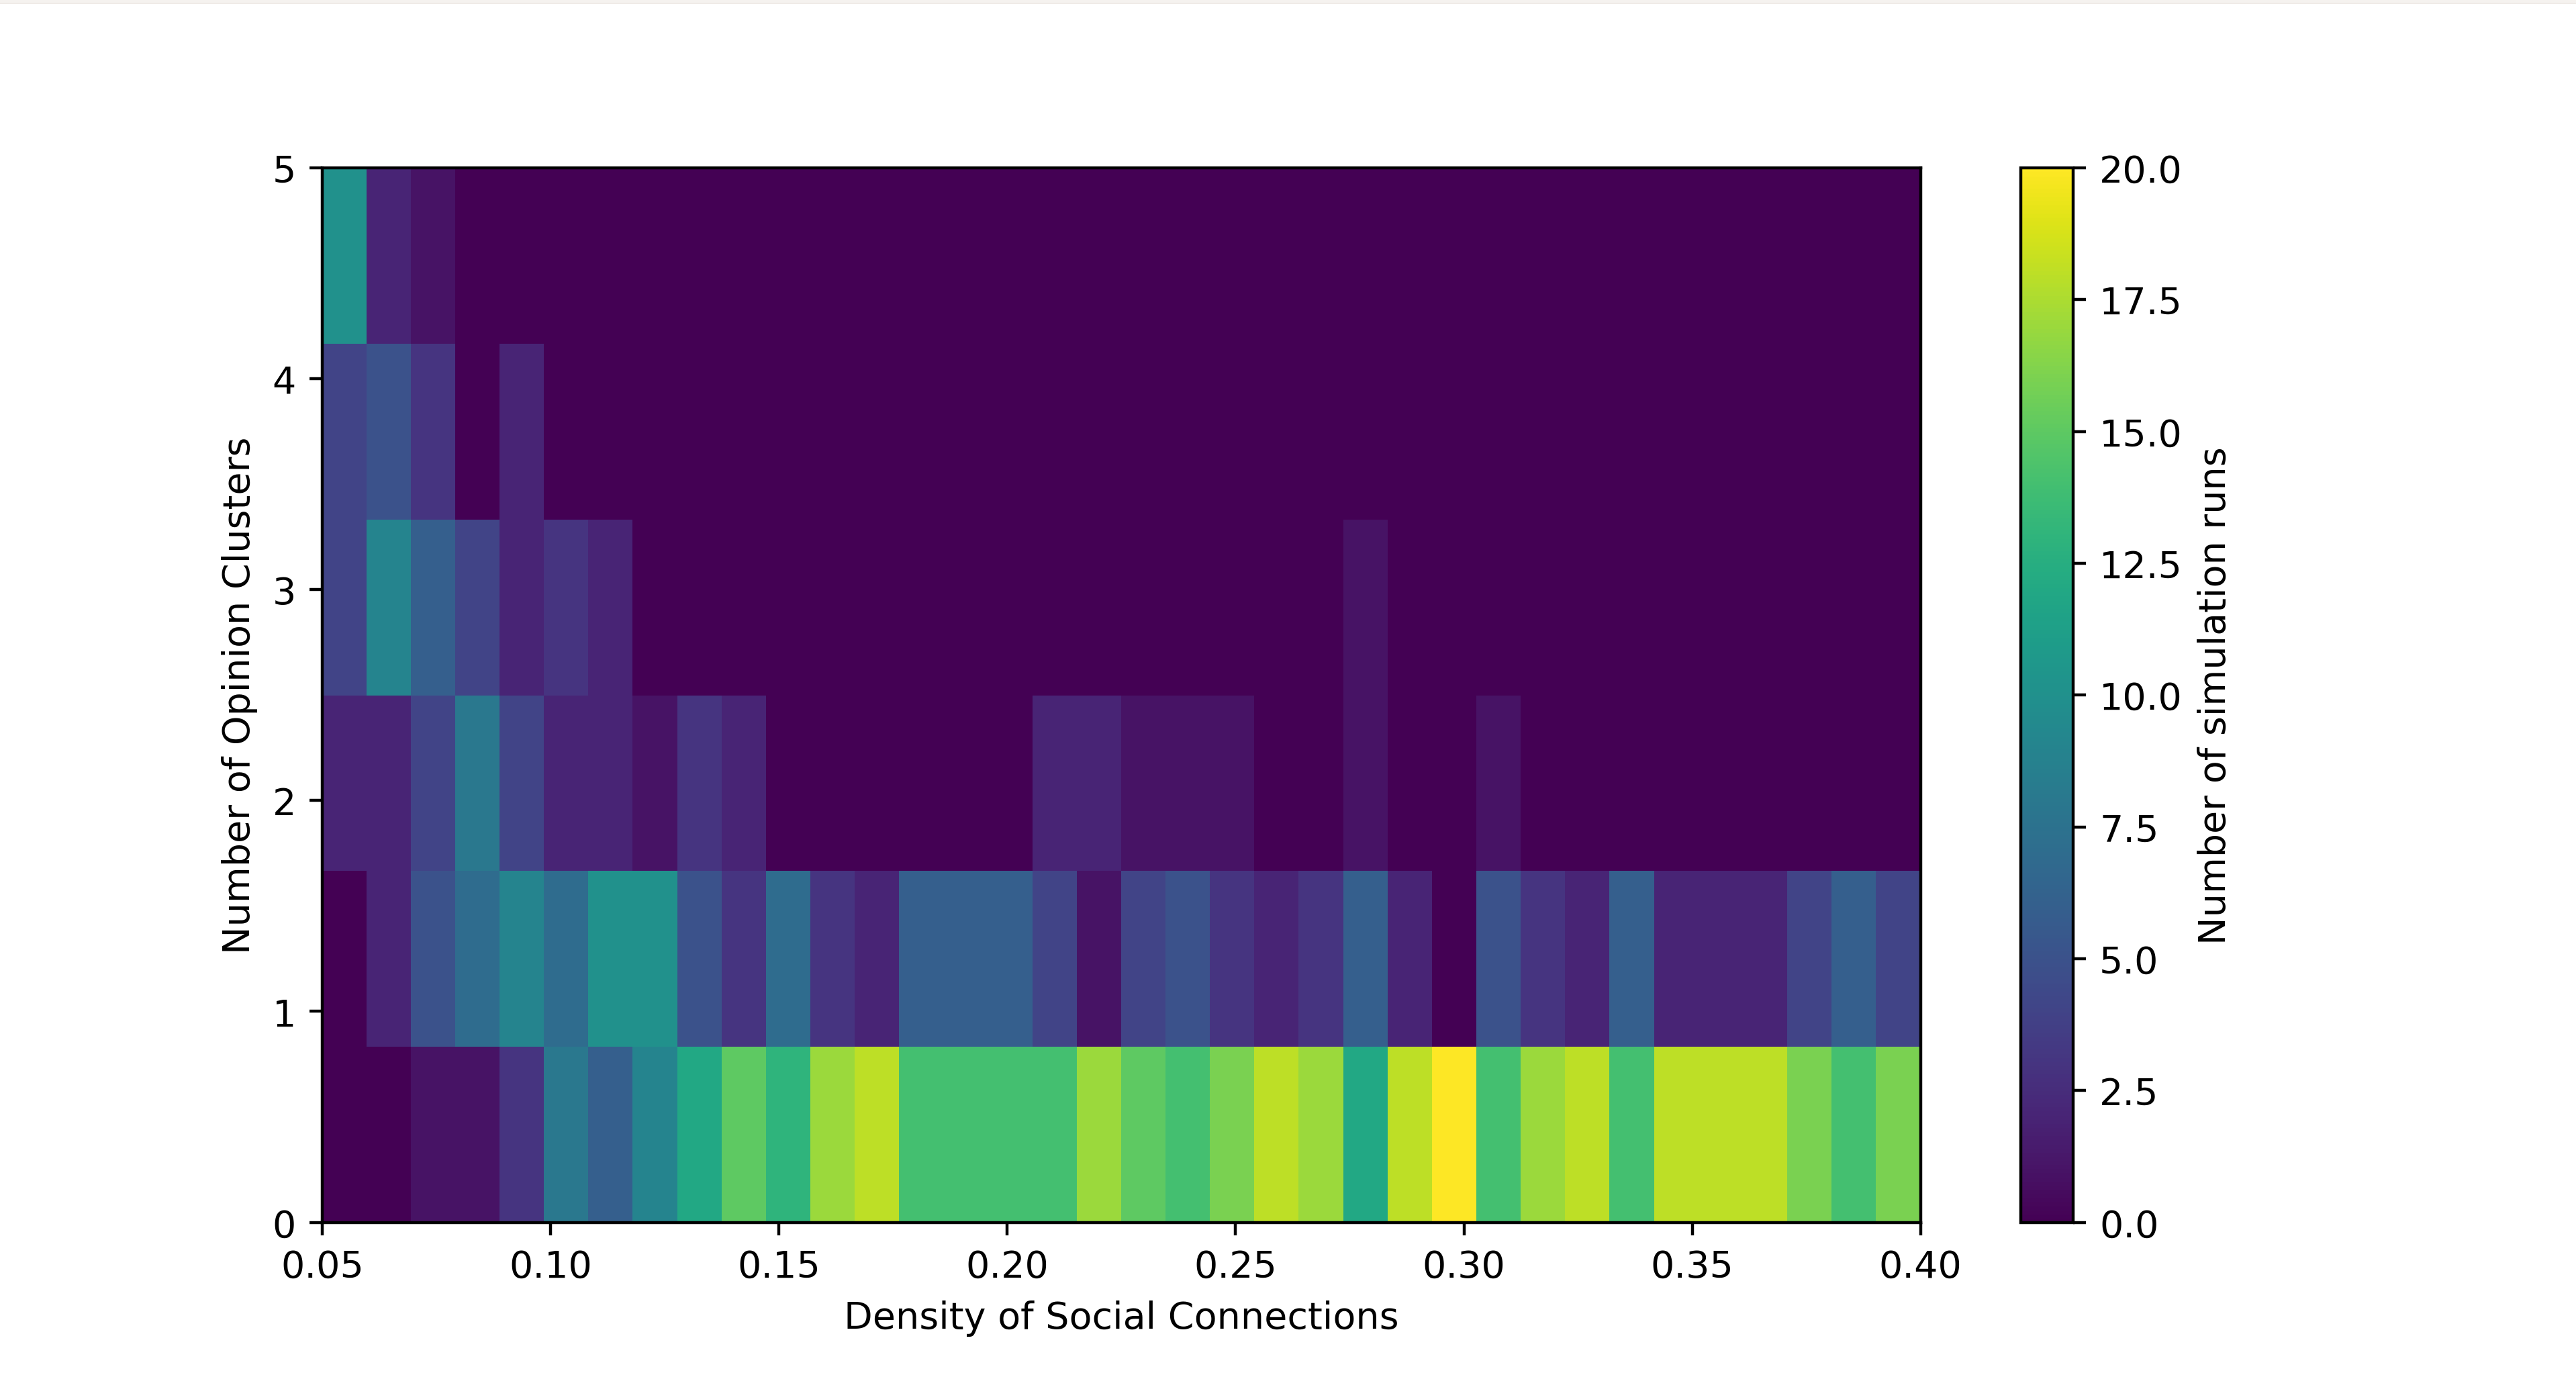
\includegraphics[width=1.0\columnwidth]{./Graphs/ClusterEdge/Cluster_edgesmall.png}
\caption{Number of Opinion Clusters and Edge Probability (0.05 - 0.40)}
\label{H2a_plot_small}
\end{figure}

The results confirm $H_{2a}$; the number of opinion clusters and edge probability have a negative relationship. I believe this may be explained by the implications of a high density for a graph of nodes. For example, when a graph of 50 nodes has a density of 0.05, the average number of social connections will be 2.5. I am able to calculate the average number of social connections by multiplying the chance there will be an edge between any two nodes (edge probability) and the number of nodes. When the edge probability, or density of the graph, increases slightly to 0.2, the average number of social connections will rise to 10 connections. As a result, the geodesic distance between two nodes decreases rapidly because each node is proportionately connected to more nodes in the graph. This may reveal why I saw that only a certain level of density is required for the number of opinion clusters to drop sharply. Undeniably, a tipping point exists with the number of opinion clusters when increasing the density of an Erd\"{o}s-R\'{e}nyi graph in the model.  

To test $H_{2b}$, I establish a model with 50 agents, 5 issues, and an edge
probability of 0.50. First, I ran a parameter sweep varying the openness
threshold from 0.05 to 0.95 to measure the impact of varying the openness
threshold on the number of opinion clusters. The results of this parameter
sweep are shown in Figure~\ref{H2b_plot_big}.

\begin{figure}
\centering
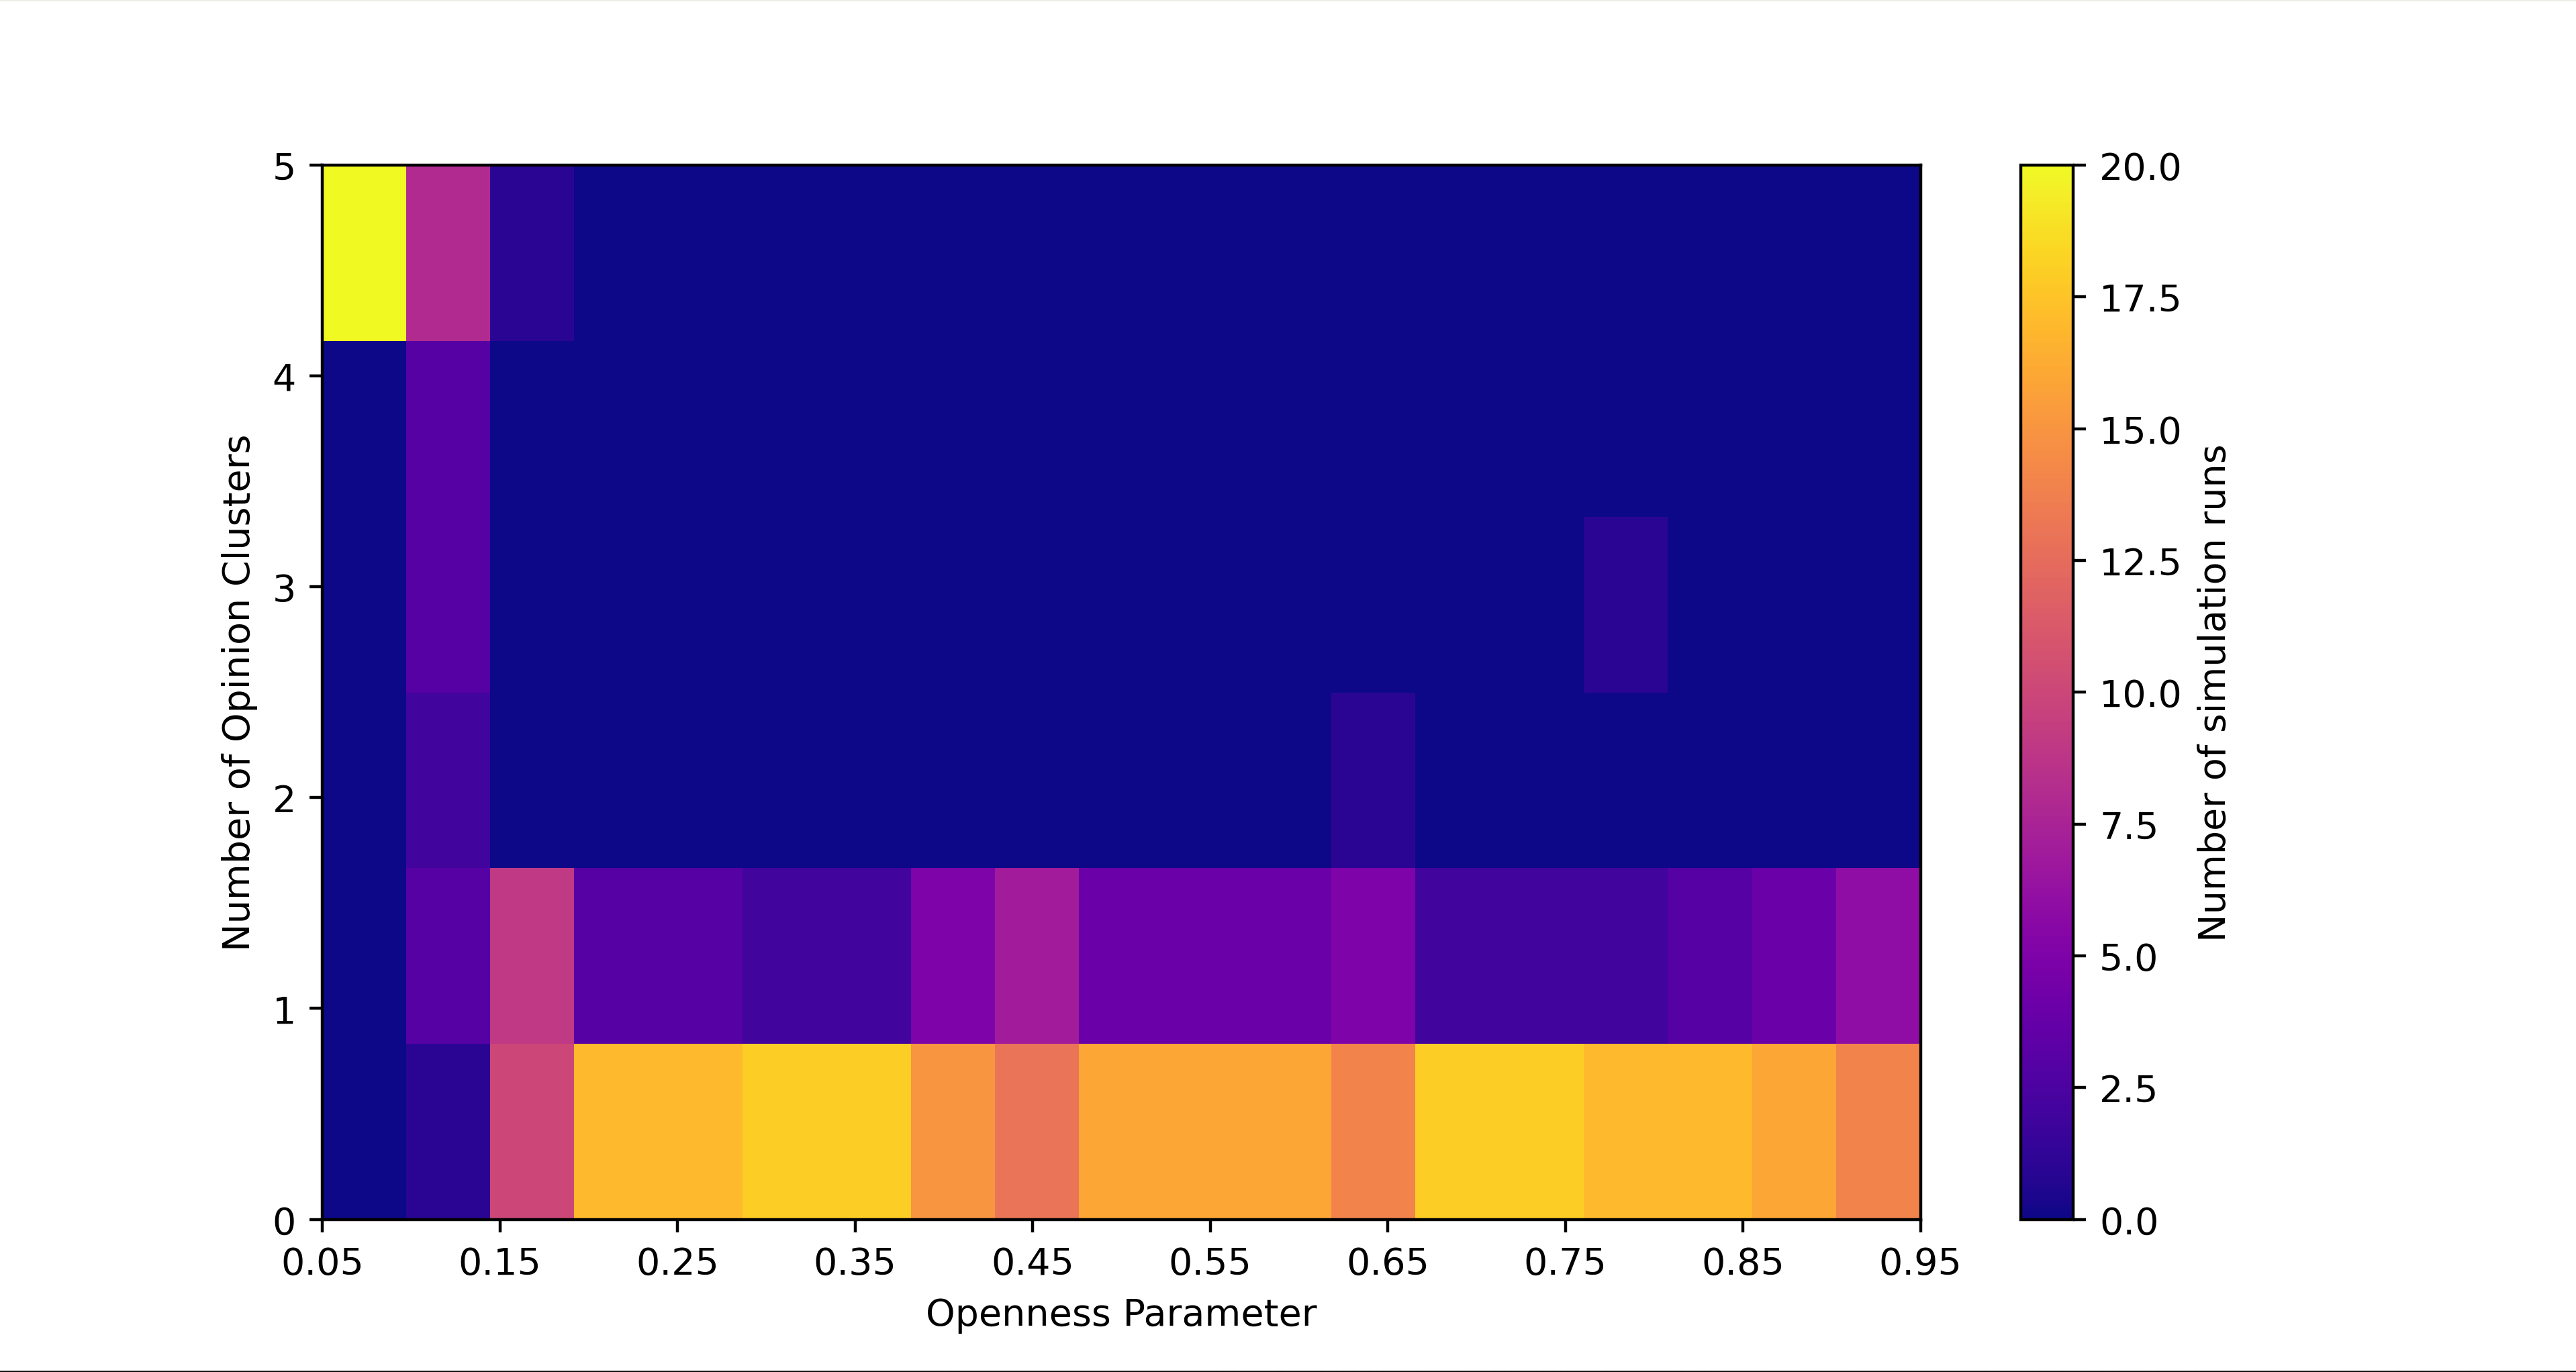
\includegraphics[width=1.0\columnwidth]{./Graphs/Cluster_openBig.png}
\caption{Number of Opinion Clusters and the Openness Threshold (0.05 - 0.95)}
\label{H2b_plot_big}
\end{figure}

I noticed that there was little to no difference between an openness threshold
of 0.5 and 0.7. However, I observed that the openness threshold had more
impact on the number of opinion clusters when the parameter was closer to 0.10.
To further explore this result, I ran another parameter sweep with 50 agents,
5 issues, an edge probability of 0.50, and a suite size of 20. This time, I
varied the openness parameter from 0.05 to 0.40. The results are depicted in
Figure~\ref{H2b_plot_small}.

\begin{figure}
\centering
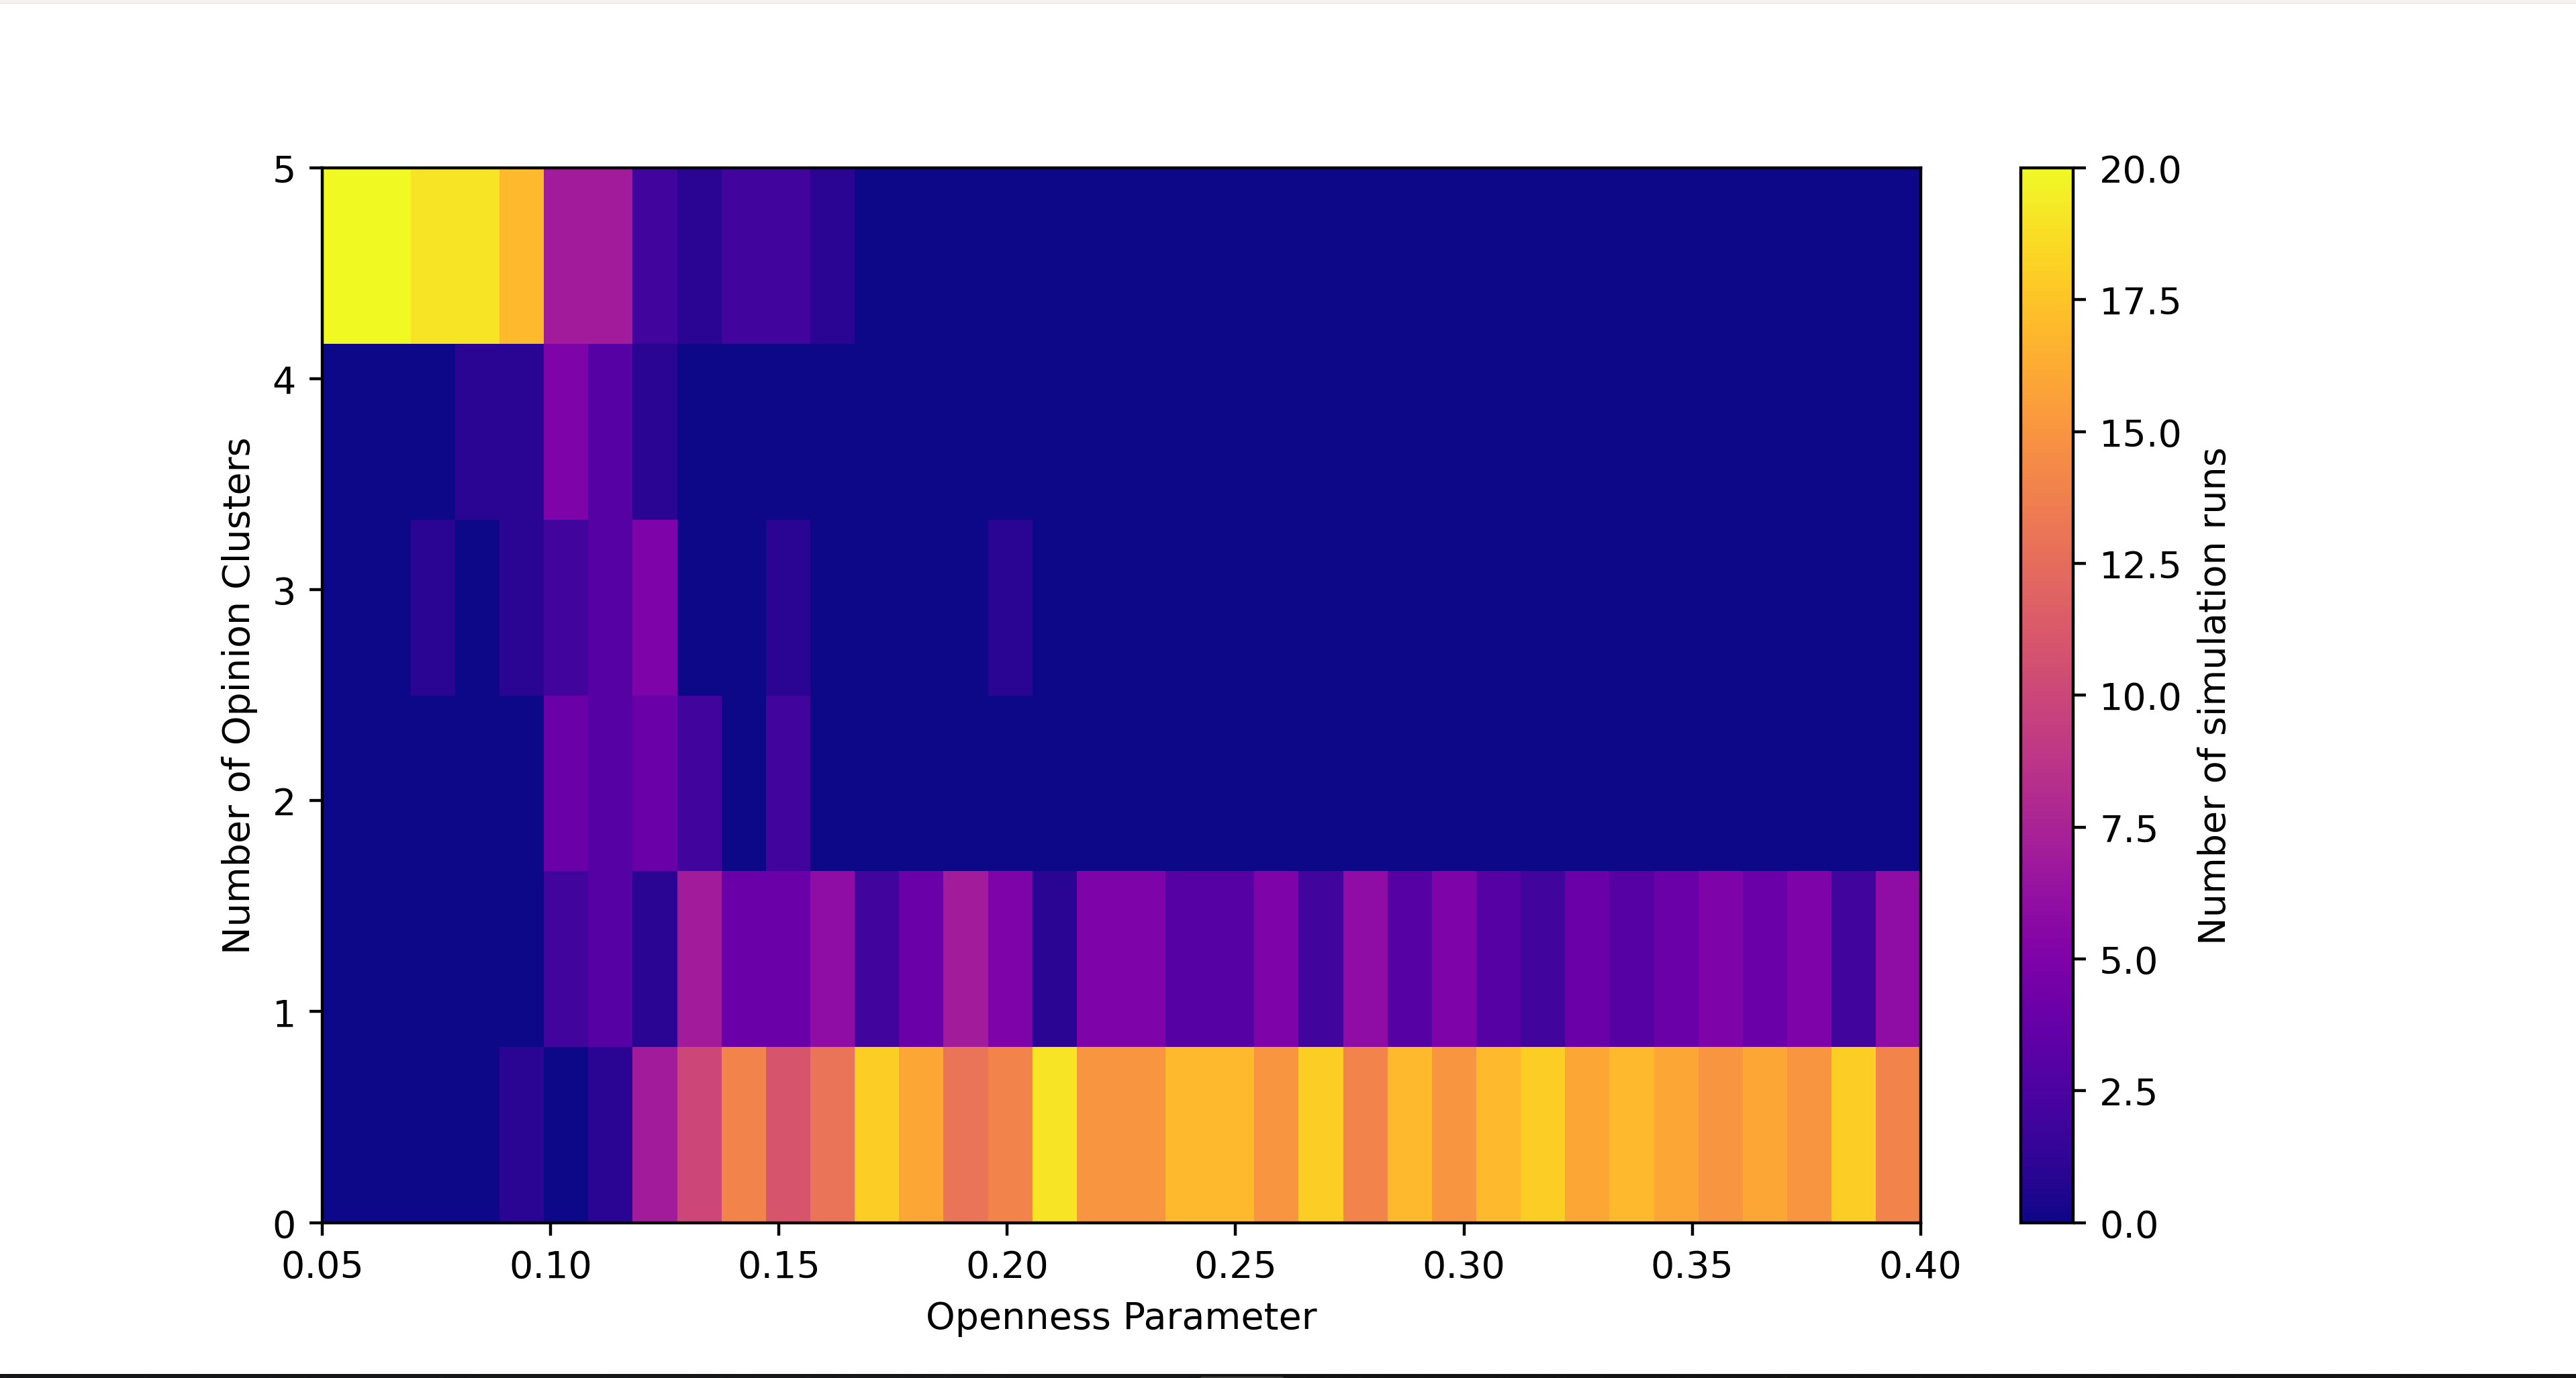
\includegraphics[width=1.0\columnwidth]{./Graphs/Cluster_opensmall.png}
\caption{Number of Opinion Clusters and Openness (0.05 - 0.40)}
\label{H2b_plot_small}
\end{figure}

This graph indicates that there is a tipping point for the openness threshold.
When the openness for agents in the model is very low, the agents did not agree
on many issues. However, as Figure~\ref{H2b_plot_small} indicates, when I
increase the openness threshold slightly, the number of opinion clusters across
the model quickly drops. As a result, I can infer that low levels of openness
in a society may induce more polarized societies. When agents in the model are
less open to distant opinions, there are more opinion clusters for any given
issue. However, the tipping point leads us to believe that slightly higher
levels of openness are sufficient to reach uniformity on a given issue for all
agents in the model. To conclude, when using the cross-issue influence
mechanism, marginally higher levels of openness led to to less polarization in
the model.

\subsection{$H_{3}$}

To test $H_{3}$, I establish a model with 100 agents, 3 issues, and an edge
probability of 0.20. The model has an openness threshold of 0.15 and a disgust threshold of 0.55. In my explanation of this result, I analyze the plots of multiple single runs of the model. 

The three plots below show what I term a census plot. The census plot shows the number of clones and anti-clones as well as the number of agent pairs that agree on one issue and two issues. The number of anti-clones represents the number of agent pairs that agree on none of the issues, and the number of clones represents the number of agent pairs that agree on every issue. This plot also has a maroon dashed line that represents the number of distinct opinion buckets. For clarity, the number of buckets is annotated on the graph once the model reaches equilibrium.

\subsubsection{Same-Issue Influence (I2)}

Figure~\ref{H3_census_I2} shows one run of the model with the combination of parameters above. The agents in this run were following the same-issue influence mechanism. 

\begin{figure}
\centering
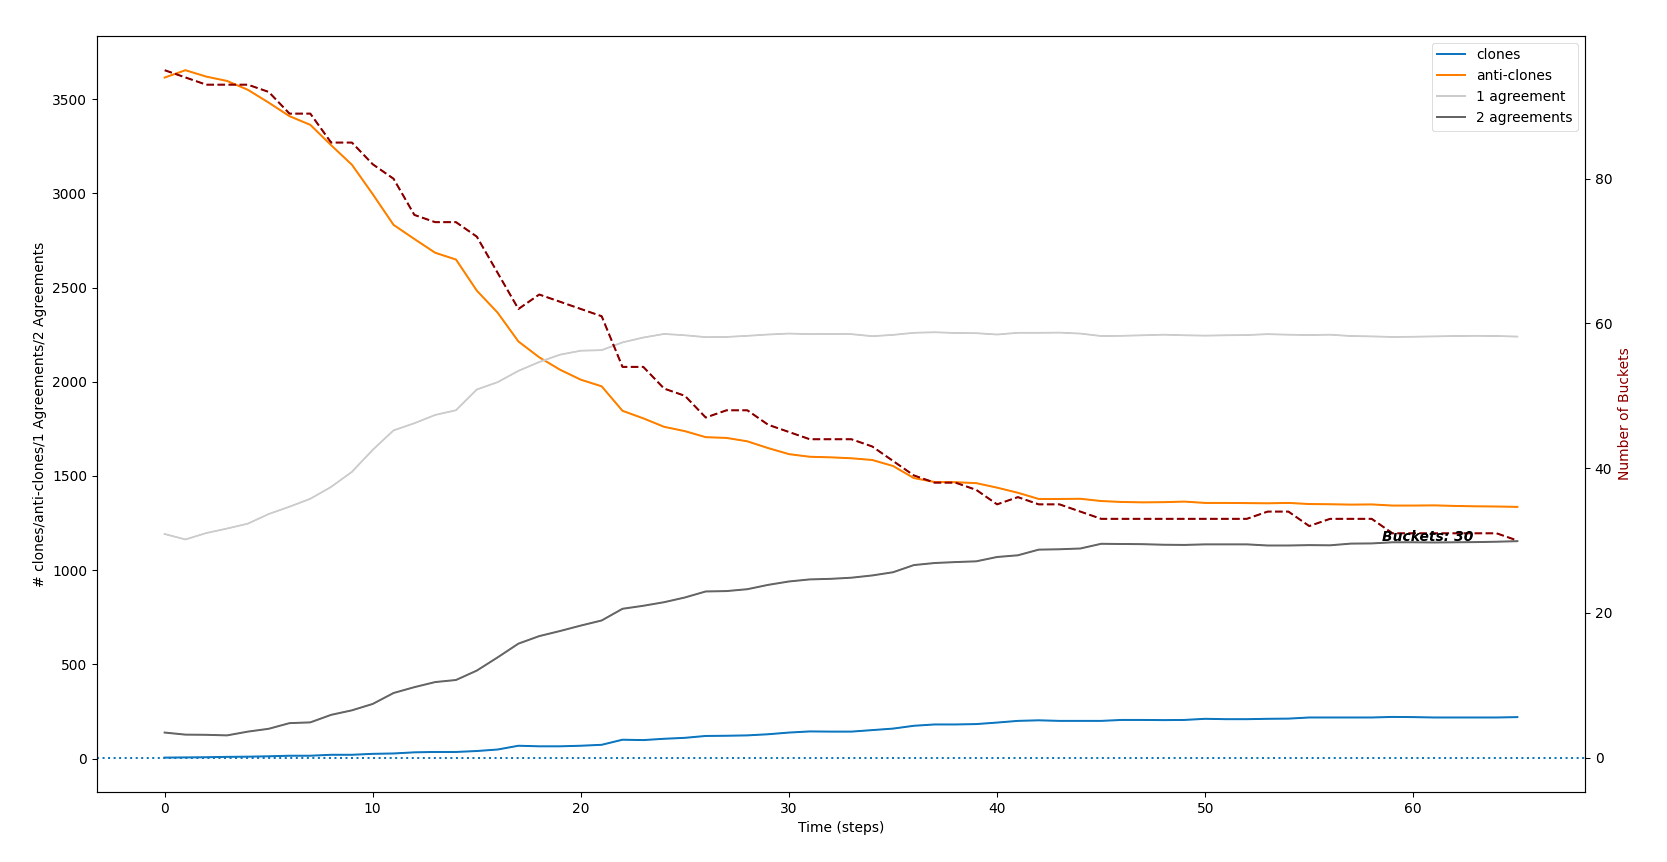
\includegraphics[width=1.0\columnwidth]{./Graphs/census3I2.png}
\caption{Number of Distinct Opinion Buckets and I2}
\label{H3_census_I2}
\end{figure}

This plot shows that as the model runs, agents influence each other and get pulled towards some consensus on the issues. The number of agent pairs that agree on one issue (shown by the light grey line) increases as does the number of agent pairs that agree on two issues (shown by the darker grey line) in the model. Additionally, the number of anticlones decreases as individuals converge to some consensus. The number of clone pairs remains low because in models where I2 is the influence mechanism, there is only marginal levels of consensus across issues. Furthermore, the number of distinct opinion buckets decreases over time. When the model is initialized, each agent is given a random opinion value for each issue, so each agent is in their own bucket at simulated time step 0. As the model runs, the number of buckets decreases from around 100 (one for each agent) to 30 buckets. This represents some consensus on the issues, but I would not call the social network in this model polarized. After examining an example plot with I2, now I turned on the CI2 mechanism.

\subsubsection{Cross-Issue Influence (CI2)}

Figure ~\ref{H3_census_CI2} shows one run of the model with the same combination of parameters defined above. However, the agents in this run were following the cross-issue influence mechanism. 

\begin{figure}
\centering
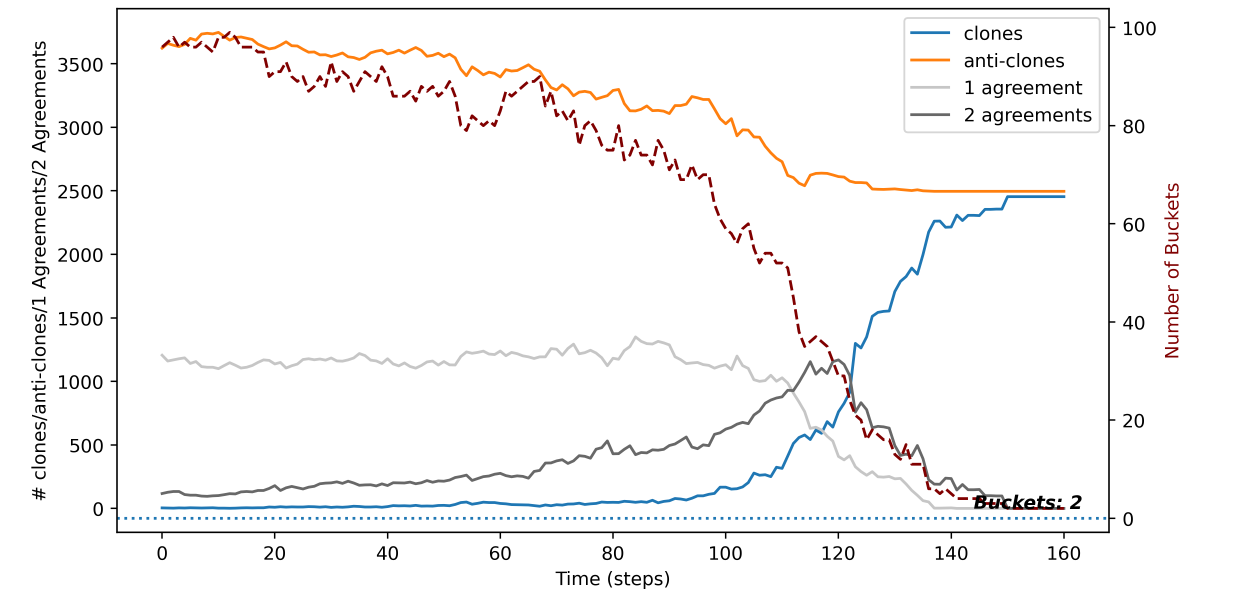
\includegraphics[width=1.0\columnwidth]{./Graphs/census3CI2.png}
\caption{Number of Distinct Opinion Buckets and CI2}
\label{H3_census_CI2}
\end{figure}

As depicted in the plot, the results of a model run with CI2 turned on are very different from the previous graph. The number of agent pairs that agree on one issue (again shown by the light grey line) increases until the number of agent pairs that agree on two issues (again shown by the darker grey line) takes over. This line increases until the number of clone pairs (represented by the blue line) rapidly begins to increase. The number of clone pairs is much higher in a model with CI2 agents compared to a model with I2 agents.  

It is important to note that if a pair of agents agrees on two out of the three issues, this pair is not counted as agreeing on one issue. This detail is a result of how the number of pairwise agreements are calculated, so the same thing happens with the number of clones taking over and the number of pairs with two agreements decreasing. Simply, if a pair agrees on two issues, they are no longer counted as agreeing on one issue.

The most interesting thing about the result shown in Figure ~\ref{H3_census_CI2} is the state of the model at equilibrium. The model starts out with each agent having randomly assigned opinion values for each issue. As a result the number of buckets is equal to the number of agents in the model because the chances of agents being in the same bucket with three randomly assigned opinion values is extremely low. Additionally, when the model is initialized, most agents are anti-clones because they are all in different buckets. However, when the model finishes running, every agent pair is either an anti-clone pair or a clone pair. Either agents are in the same bucket for each issue, or they disagree on every issue. The number of opinion buckets at equilibrium plummets to only two buckets compared to the thirty buckets at equilibrium for Figure ~\ref{H3_census_I2}. The social network depicted in Figure ~\ref{H3_census_CI2} is much more issue aligned, and therefore polarized, than the network behind the results shown in ~\ref{H3_census_I2}. With every other parameter being held constant besides the influence mechanism, I am able to attribute the increased degree of issue alignment in this society to the CI2 mechanism. 

Although this is only one example of a model where agents follow the CI2 mechanism, the decreased number of buckets was consistent across many parameter suites. Regardless of the values for the openness threshold and disgust threshold, the number of distinct opinion buckets in a society with agents following the CI2 mechanism was much lower than a society where agents follow the I2 mechanism. The average number of buckets for a large sweep of the openness and disgust thresholds with CI2 turned on was 2.61, and the average number of buckets was 21.45 sweeping over the same values of the openness and disgust threshold with CI2 turned off (I2).         

\subsubsection{Number of Distinct Opinion Buckets with Increased Issues}

One question that I had when analyzing my results was: what would the behavior of the model look like if I increased the number of issues? One advantage of the way I designed my code base is the modularity and flexibility of the model. Changing the number of issues each agent has in the model is a one line change, so I was able to easily initialize a model with 10 issues rather than only three. Then, I plotted the same census plot like Figure ~\ref{H3_census_I2} and Figure ~\ref{H3_census_CI2}. 

I initialized a model with 100 agents, an edge probability of 0.20, an openness threshold of 0.10, a disgust threshold of 0.55, and 10 issues for each agent. The result of running this model to equilibrium is shown below in Figure ~\ref{H3_census10_CI2}. 

\begin{figure}
\centering
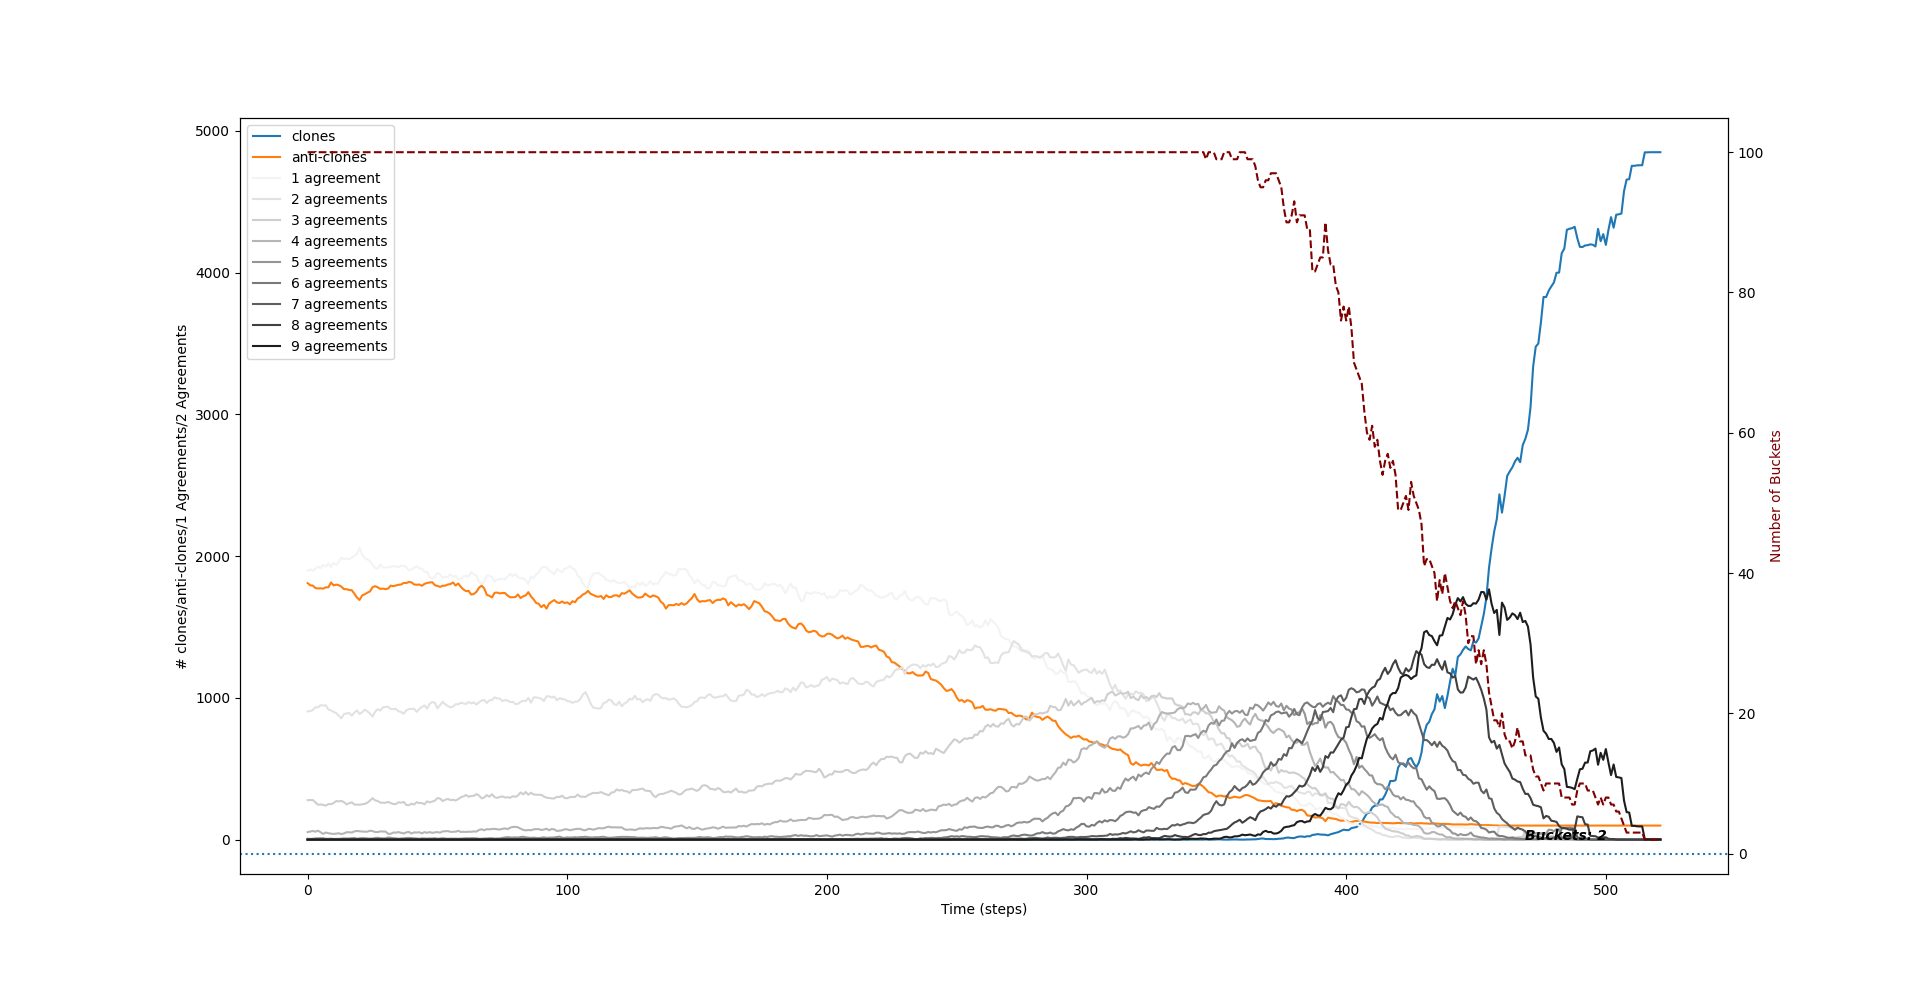
\includegraphics[width=1.0\columnwidth]{./Graphs/census10CI2.png}
\caption{Number of Distinct Opinion Buckets and CI2 with 10 Issues}
\label{H3_census10_CI2}
\end{figure}

On this plot, as the number of agreements increases, the line representing this number will get darker. The lightest grey line represents the number of agent pairs that agree on one issue, and the darkest grey line represents the number of agent pairs that agree on nine out of the ten issues. The number of anti-clone and clone pair lines remain the same color as they were on other plots. 

As shown in the Figure ~\ref{H3_census10_CI2}, even with a large number of issues, the model still converges to a relatively low number of distinct opinion buckets. With ten issues, there are more possible sets of opinion values compared to a model with only three issues, so it is more impressive to me that the ten issue model is still able to converge to a low number of opinion buckets. 

It is also interesting to look at the trend of the number of distinct opinion buckets with the number of agent pairwise agreements. For around 350 simulated time steps, the number of distinct opinion buckets does not change. However, there is a steep tipping point where the number of distinct opinion buckets quickly drops to only two. Before the number of buckets decreases, the agents in the society are increasingly separating and agreeing on more and more issues. This can be seen through each darker grey line peaking after the previous line. What results is a snowball-type effect on the plot where eventually the number of clones increases rapidly. Similar to the model with only three issues, at equilibrium, all agents are either anti-clones or clones. To me, this again represents a polarized society where agents have aligned into only two distinct opinion buckets.   
